\documentclass{standalone}
\usepackage{tikz}
\usepackage{standalone}
\begin{document}
	
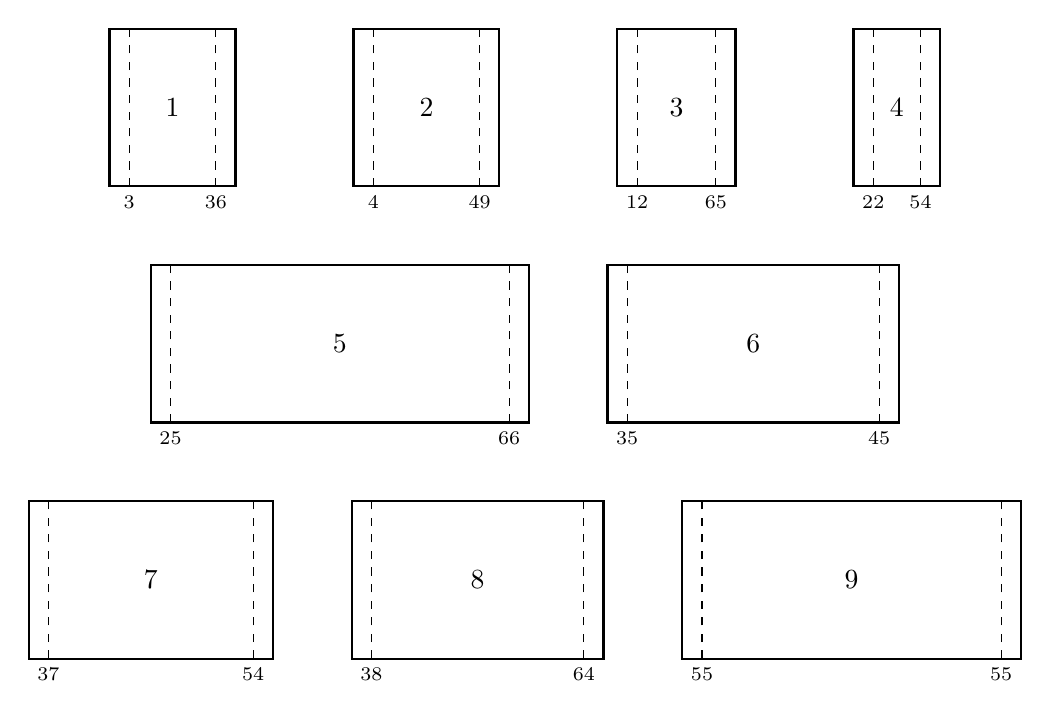
\begin{tikzpicture}
%\draw [help lines] (-.5,-2) grid (14, 9.5);

\draw [thick] (0,0) rectangle (3.1,2);
\draw [dashed] (0.25,0) -- (0.25,2);
\draw [dashed] (2.85,0) -- (2.85,2);
\node [below] at (0.25,0) {\scriptsize $37$};
\node [below] at (2.85,0) {\scriptsize $54$};
\node at (1.55, 1) {7};


\draw [thick] (4.1,0) rectangle (7.3,2);
\draw [dashed] (4.35,0) -- (4.35,2);
\draw [dashed] (7.05,0) -- (7.05,2);
\node [below] at (4.35,0) {\scriptsize $38$};
\node [below] at (7.05,0) {\scriptsize $64$};
\node at (5.7, 1) {8};


\draw [thick] (8.3,0) rectangle (12.6,2);
\draw [dashed] (8.55,0) -- (8.55,2);
\draw [dashed] (12.35,0) -- (12.35,2);
\node [below] at (8.55,0) {\scriptsize $55$};
\node [below] at (12.35,0) {\scriptsize $55$};
\node at (10.45, 1) {9};
%%%



\draw [thick] (1.55,3) rectangle (6.35,5);
\draw [dashed] (1.8,3) -- (1.8,5);
\draw [dashed] (6.1,3) -- (6.1,5);
\node [below] at (1.8,3) {\scriptsize $25$};
\node [below] at (6.1,3) {\scriptsize $66$};
\node at (3.95, 4) {5};


\draw [thick] (7.35,3) rectangle (11.05,5);
\draw [dashed] (7.6,3) -- (7.6,5);
\draw [dashed] (10.8,3) -- (10.8,5);
\node [below] at (7.6,3) {\scriptsize $35$};
\node [below] at (10.8,3) {\scriptsize $45$};
\node at (9.2, 4) {6};
%%%


\draw [thick] (1.025,6) rectangle (2.625,8);
\draw [dashed] (1.275,6) -- (1.275,8);
\draw [dashed] (2.375,6) -- (2.375,8);
\node [below] at (1.275,6) {\scriptsize $3$};
\node [below] at (2.375,6) {\scriptsize $36$};
\node at (1.825, 7) {1};


\draw [thick] (4.125,6) rectangle (5.975,8);
\draw [dashed] (4.375,6) -- (4.375,8);
\draw [dashed] (5.725,6) -- (5.725,8);
\node [below] at (4.375,6) {\scriptsize $4$};
\node [below] at (5.725,6) {\scriptsize $49$};
\node at (5.05, 7) {2};


\draw [thick] (7.475,6) rectangle (8.975,8);
\draw [dashed] (7.725,6) -- (7.725,8);
\draw [dashed] (8.725,6) -- (8.725,8);
\node [below] at (7.725,6) {\scriptsize $12$};
\node [below] at (8.725,6) {\scriptsize $65$};
\node at (8.226, 7) {3};


\draw [thick] (10.475,6) rectangle (11.575,8);
\draw [dashed] (10.725,6) -- (10.725,8);
\draw [dashed] (11.325,6) -- (11.325,8);
\node [below] at (10.725,6) {\scriptsize $22$};
\node [below] at (11.325,6) {\scriptsize $54$};
\node at (11.025, 7) {4};



\end{tikzpicture}
	
\end{document}